\begin{figure}[ht]
\centering
\resizebox{\textwidth}{!}{%
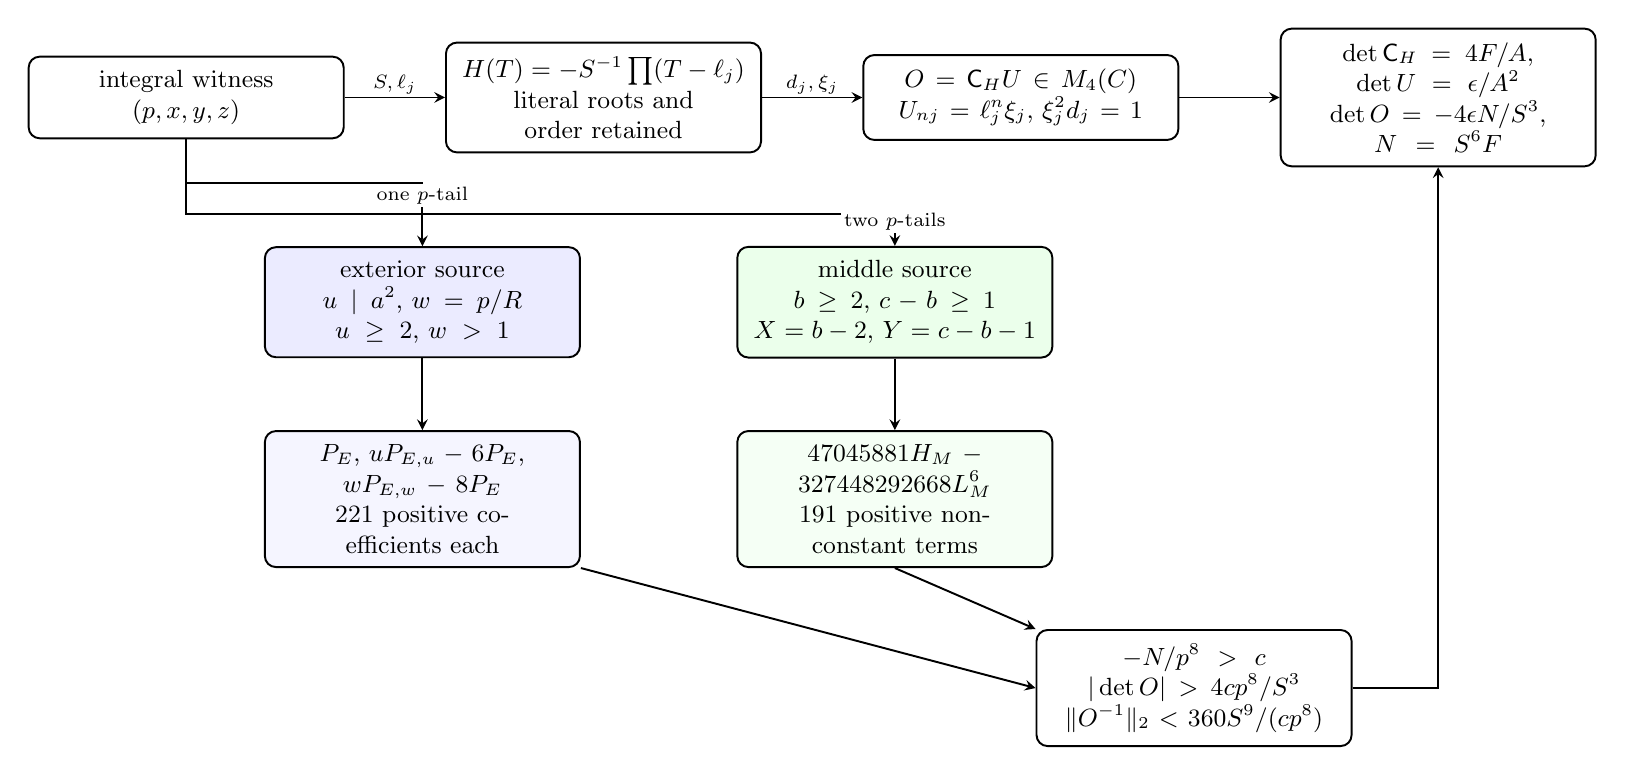
\begin{tikzpicture}[
  font=\small,>=stealth,
  box/.style={draw,rounded corners,align=center,inner sep=5pt,minimum height=1.0cm,text width=3.65cm},
  every path/.style={line width=.7pt}]
  \node[box] (w) at (0,0) {integral witness\\$(p,x,y,z)$};
  \node[box] (h) at (5.3,0) {$H(T)=-S^{-1}\prod(T-\ell_j)$\\literal roots and order retained};
  \node[box] (o) at (10.6,0) {$O=\mathsf C_HU\in M_4(\mathbb C)$\\$U_{nj}=\ell_j^n\xi_j$, $\xi_j^2d_j=1$};
  \node[box] (d) at (15.9,0) {$\det\mathsf C_H=4F/A$, $\det U=\epsilon/A^2$\\$\det O=-4\epsilon\mathfrak N/S^3$, $\mathfrak N=S^6F$};
  \draw[->] (w) -- node[above,font=\scriptsize,fill=white,inner sep=1pt] {$S,\ell_j$} (h);
  \draw[->] (h) -- node[above,font=\scriptsize,fill=white,inner sep=1pt] {$d_j,\xi_j$} (o);
  \draw[->] (o) -- (d);

  \node[box,fill=blue!8] (e) at (3.0,-2.6)
    {exterior source\\$u\mid a^2$, $w=p/R$\\$u\ge2$, $w>1$};
  \node[box,fill=green!8] (m) at (9.0,-2.6)
    {middle source\\$b\ge2$, $c-b\ge1$\\$X=b-2$, $Y=c-b-1$};
  \node[box,fill=blue!4] (ec) at (3.0,-5.1)
    {$P_E$, $uP_{E,u}-6P_E$, $wP_{E,w}-8P_E$\\$221$ positive coefficients each};
  \node[box,fill=green!4] (mc) at (9.0,-5.1)
    {$47045881H_M-327448292668L_M^6$\\$191$ positive nonconstant terms};
  \node[box] (c) at (12.8,-7.5)
    {$-\mathfrak N/p^8>c$\\$|\det O|>4cp^8/S^3$\\$\|O^{-1}\|_2<360S^9/(cp^8)$};
  \draw[->] (w.south) -- ++(0,-.55) -| node[pos=.70,above,font=\scriptsize,fill=white,inner sep=1pt] {one $p$-tail} (e.north);
  \draw[->] (w.south) -- ++(0,-.95) -| node[pos=.82,above,font=\scriptsize,fill=white,inner sep=1pt] {two $p$-tails} (m.north);
  \draw[->] (e) -- (ec);
  \draw[->] (m) -- (mc);
  \draw[->] (ec.south east) -- (c.west);
  \draw[->] (mc.south) -- (c.north west);
  \draw[->] (c.east) -| (d.south);
\end{tikzpicture}
}%
\caption{Typed route from a positive integral witness to the receiver bound.
The two arithmetic branches exhaust the witness domain.  The root labels,
square-root signs, complex coefficient map and determinant phase are retained;
the polynomial certificates control only the final real scalar
$-\mathfrak N/p^8$.}
\label{fig:determinant-mechanism}
\end{figure}
